\newpage
\section{Housing}
The Housing was designed in OpenSCAD.\
a very helpfull reference for the OpenSCAD syntax was\
\url{https://en.wikibooks.org/wiki/OpenSCAD_User_Manual/Transformations}

\subsection{Housing 1}
The Housing was printed by the TOOM Printing Service as SLS in PLA.\
Sadly all the surfaces are not really smooth, therefore the Buttons are working very bad.\
I tried to glue in the glass with superglue, but the glue dried out white, this looks really bad :-(\

\subsection{Plans for Housing 2}
The next housing should be produced via SLA with transparent Resin, so no glass for Protection is needed, 
since the resin could be used.
\subsubsection{Problems while printing with SLA}
It turns out, that there is no completely transparent Resin available. All of them get a yellow color sooner or later.
So it is not really beautiful as a glass.

\subsection{Housing 2}
A friend told me that most of the time the resin will not reflect light equally in every spot, therefore i decided to order a PCB without glass and do the mounting of the glass with very tight tolerances and a rim on the top edge.\
this worked out extremely well.\
Another goal was to make the second Housing slim, because the first one was very bulky. With a bit of optimization is was possible to integrate the bottom plate completely in the housing. The overall thicknes was reduced from about 15mm to 9.4mm with the 1mm PCB or 10mm with the new 1.6mm PCB.\
For the PCB to tightly fit in either the Housing has to get some aditional holes or at least the Battery clip has to be modified.\
\begin{center}
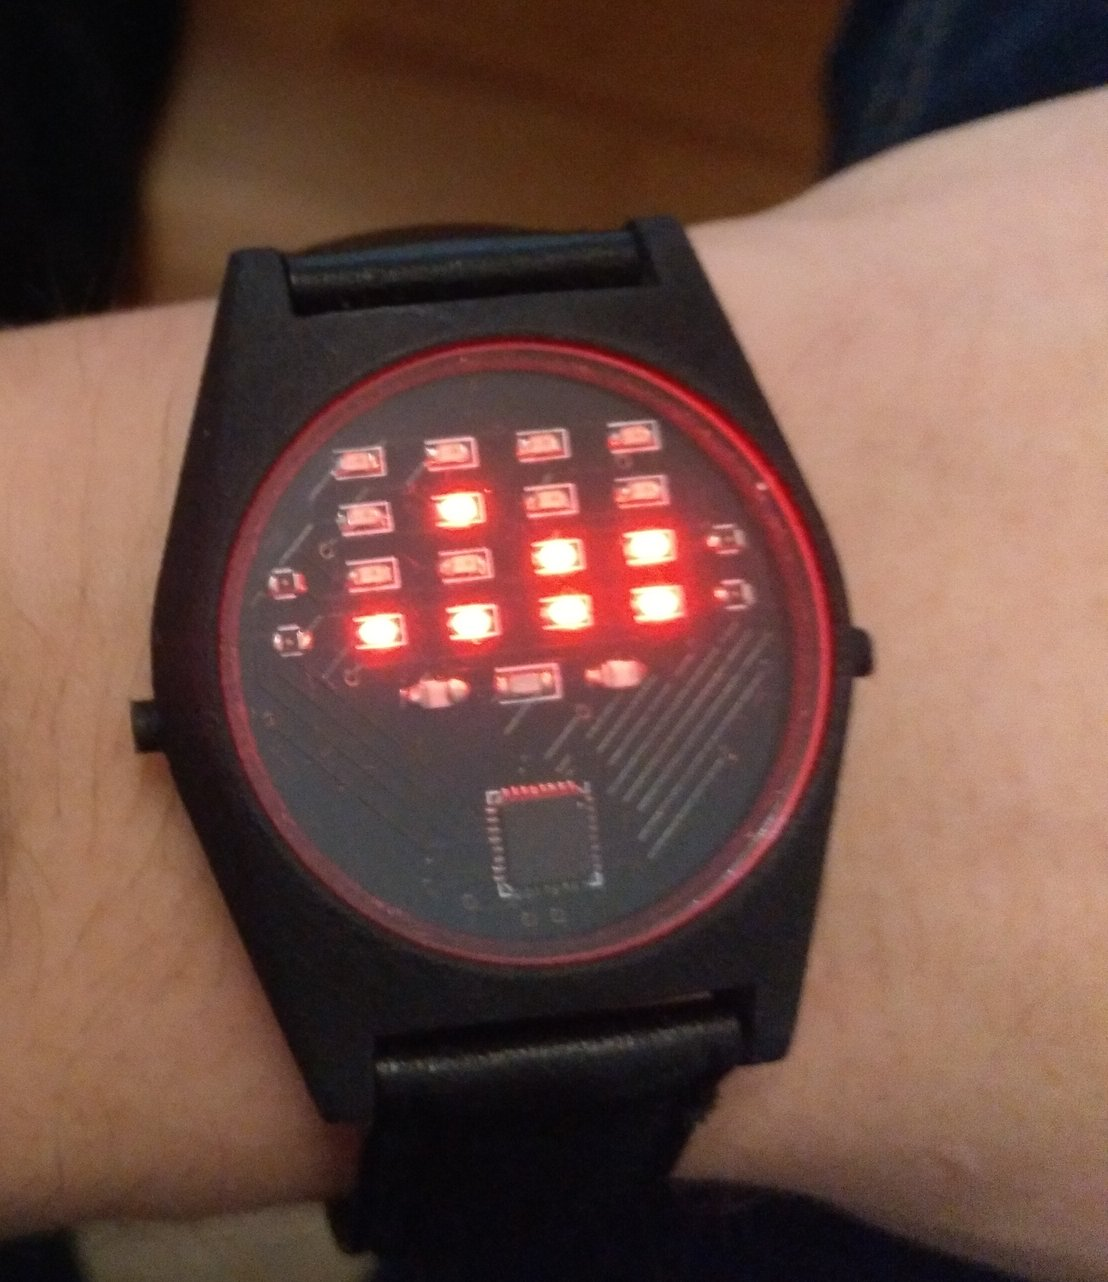
\includegraphics[width=0.45\textwidth]{../Pictures/Housing2.jpg} 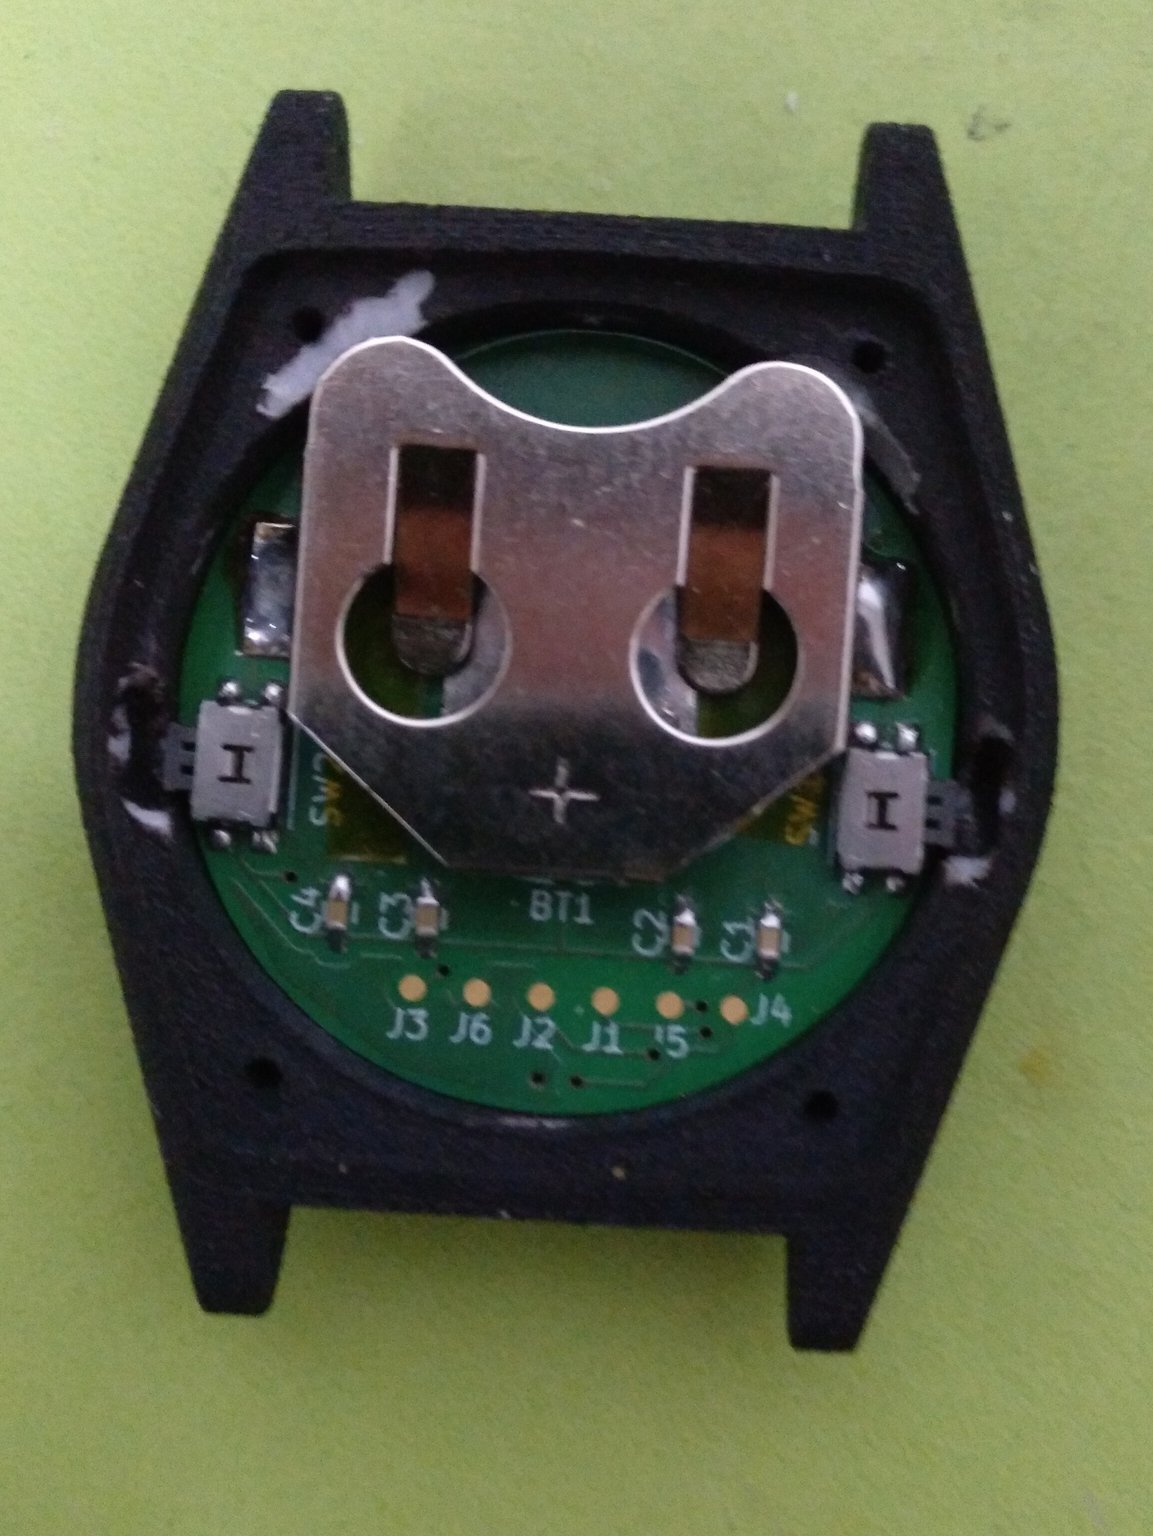
\includegraphics[width=0.45\textwidth]{../Pictures/Housing3b.jpg}
\end{center}
